\documentclass[12pt,letterpaper]{article}
\usepackage{graphicx,textcomp}
\usepackage{natbib}
\usepackage{setspace}
\usepackage{fullpage}
\usepackage{color}
\usepackage[reqno]{amsmath}
\usepackage{amsthm}
\usepackage{fancyvrb}
\usepackage{amssymb,enumerate}
\usepackage[all]{xy}
\usepackage{endnotes}
\usepackage{lscape}
\newtheorem{com}{Comment}
\usepackage{float}
\usepackage{hyperref}
\newtheorem{lem} {Lemma}
\newtheorem{prop}{Proposition}
\newtheorem{thm}{Theorem}
\newtheorem{defn}{Definition}
\newtheorem{cor}{Corollary}
\newtheorem{obs}{Observation}
\usepackage[compact]{titlesec}
\usepackage{dcolumn}
\usepackage{tikz}
\usetikzlibrary{arrows}
\usepackage{multirow}
\usepackage{xcolor}
\newcolumntype{.}{D{.}{.}{-1}}
\newcolumntype{d}[1]{D{.}{.}{#1}}
\definecolor{light-gray}{gray}{0.65}
\usepackage{url}
\usepackage{listings}
\usepackage{color}

\definecolor{codegreen}{rgb}{0,0.6,0}
\definecolor{codegray}{rgb}{0.5,0.5,0.5}
\definecolor{codepurple}{rgb}{0.58,0,0.82}
\definecolor{backcolour}{rgb}{0.95,0.95,0.92}

\lstdefinestyle{mystyle}{
	backgroundcolor=\color{backcolour},   
	commentstyle=\color{codegreen},
	keywordstyle=\color{magenta},
	numberstyle=\tiny\color{codegray},
	stringstyle=\color{codepurple},
	basicstyle=\footnotesize,
	breakatwhitespace=false,         
	breaklines=true,                 
	captionpos=b,                    
	keepspaces=true,                 
	numbers=left,                    
	numbersep=5pt,                  
	showspaces=false,                
	showstringspaces=false,
	showtabs=false,                  
	tabsize=2
}
\lstset{style=mystyle}
\newcommand{\Sref}[1]{Section~\ref{#1}}
\newtheorem{hyp}{Hypothesis}

\title{Problem Set 3}
\date{Due: November 19, 2022}
\author{Applied Stats/Quant Methods 1}


\begin{document}
	\maketitle
	\section*{Instructions}
	\begin{itemize}
		\item Please show your work! You may lose points by simply writing in the answer. If the problem requires you to execute commands in \texttt{R}, please include the code you used to get your answers. Please also include the \texttt{.R} file that contains your code. If you are not sure if work needs to be shown for a particular problem, please ask.
	\item Your homework should be submitted electronically on GitHub.
	\item This problem set is due before 23:59 on Sunday November 19, 2023. No late assignments will be accepted.

	\end{itemize}

		\vspace{.25cm}
	
\noindent In this problem set, you will run several regressions and create an add variable plot (see the lecture slides) in \texttt{R} using the \texttt{incumbents\_subset.csv} dataset. Include all of your code.

	\vspace{.5cm}
\section*{Question 1}
\vspace{.25cm}
\noindent We are interested in knowing how the difference in campaign spending between incumbent and challenger affects the incumbent's vote share. 
	\begin{enumerate}
		\item Run a regression where the outcome variable is \texttt{voteshare} and the explanatory variable is \texttt{difflog}.	\vspace{1cm}
		
		\begin{lstlisting}[language=R, caption={Regression Model 1 in R}, label={lst:regression_model}]
			# Run regression model in R
			Regression_1 <- lm(voteshare ~ difflog, data = incumbents_subset)
			
			# Get summary of model with coefficient estimates
			summary(Regression_1)
		\end{lstlisting}		
			
		\begin{verbatim}
		Coefficients:
		Estimate Std. Error t value Pr(>|t|)    
		(Intercept) 0.579031   0.002251  257.19   <2e-16 ***
		difflog     0.041666   0.000968   43.04   <2e-16 ***
		---
		Signif. codes:  0 ‘***’ 0.001 ‘**’ 0.01 ‘*’ 0.05 ‘.’ 0.1 ‘ ’ 1
		
		Residual standard error: 0.07867 on 3191 degrees of freedom
		Multiple R-squared:  0.3673,	Adjusted R-squared:  0.3671 
		F-statistic:  1853 on 1 and 3191 DF,  p-value: < 2.2e-16
			\end{verbatim}
			
		\item Make a scatterplot of the two variables and add the regression line. 	\vspace{7cm}
		
		\vspace{-7cm}
		
		\begin{lstlisting}[language=R, caption={Scatterplot 1 code in R}, label={lst:regression_model}]
			# Create a scatterplot with regression line
			ScatterplotRegression1<-ggplot(incumbents_subset, 
			aes(x = difflog, y = voteshare)) +
			geom_point() +
			geom_smooth(method = "lm", se = FALSE, color = "blue") +
			labs(title = "Scatterplot of Regression 1",
			x = "Difference in Campaign Spending (difflog)",
			y = "Incumbent Vote Share")
			
			# Save Scatterplot as an image
			ggsave("Scatterplot_of_Regression_1.pdf", 
			plot = ScatterplotRegression1, 
			width = 6, height = 4, units = "in")
		\end{lstlisting}	
		
						
		\begin{figure}[H]
			\centering
			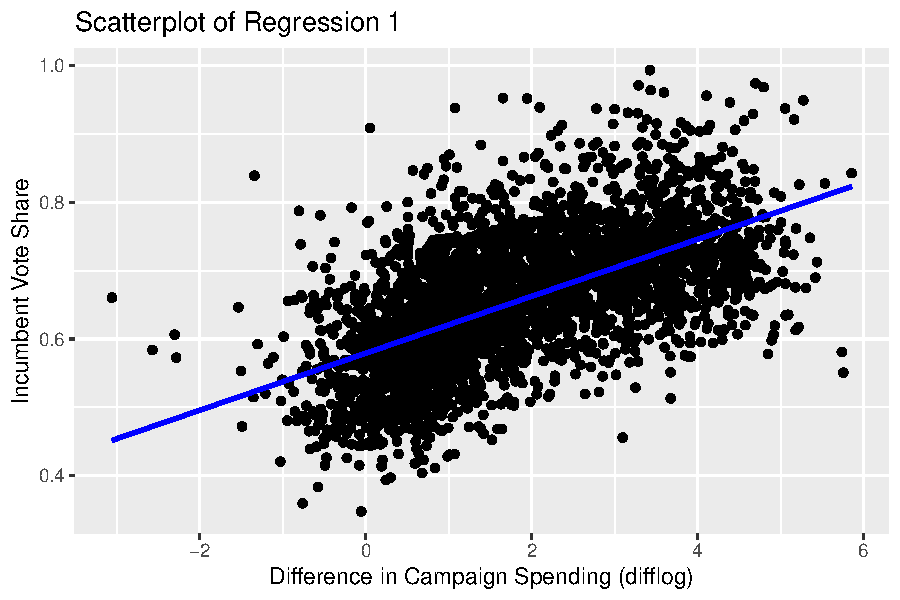
\includegraphics[width=0.85\textwidth]{Scatterplot_of_Regression_1.pdf}
			\caption{Scatterplot of Regression 1}
			\label{fig:scatterplot_regression1}
		\end{figure}

        
		\item Save the residuals of the model in a separate object.	\vspace{7cm}
		\vspace{-7cm}
		
		\begin{lstlisting}
		Save the residuals of the model in a separate object (R).
		residuals_1 <- resid(Regression_1)
		\end{lstlisting}
			
		\item Write the prediction equation.
		
		\begin{align*}
			Y &= B_0 + B_1 \quad \text{(Linear Regression Model)} \\
			\text{Predicted Incumbent voteshare} &= 0.579031 + 0.041666 \times \text{difflog} \quad \text{(Specific coefficients)}
		\end{align*}
				
	\end{enumerate}
	
	
	
\newpage

\section*{Question 2}
\noindent We are interested in knowing how the difference between incumbent and challenger's spending and the vote share of the presidential candidate of the incumbent's party are related.	\vspace{.25cm}
	\begin{enumerate}
		\item Run a regression where the outcome variable is \texttt{presvote} and the explanatory variable is \texttt{difflog}.	\vspace{1cm}
		
		\begin{lstlisting}[language=R, caption={Regression Model 2 in R}, label={lst:regression_model}]
		#Run a regression model where the outcome variable is presvote and 
		the explanatory variable is difflog.
		Regression_2 <- lm(presvote ~ difflog, data = incumbents_subset)
	
		# Get summary of model with coefficient estimates
		summary(Regression_2)
		\end{lstlisting}		
		
		
		\begin{verbatim}
		Coefficients:
		Estimate Std. Error t value Pr(>|t|)    
		(Intercept) 0.507583   0.003161  160.60   <2e-16 ***
		difflog     0.023837   0.001359   17.54   <2e-16 ***
		---
		Signif. codes:  0 ‘***’ 0.001 ‘**’ 0.01 ‘*’ 0.05 ‘.’ 0.1 ‘ ’ 1
		
		Residual standard error: 0.1104 on 3191 degrees of freedom
		Multiple R-squared:  0.08795,	Adjusted R-squared:  0.08767 
		F-statistic: 307.7 on 1 and 3191 DF,  p-value: < 2.2e-16
	\end{verbatim}
		
		\newpage
		\item Make a scatterplot of the two variables and add the regression line. 	\vspace{1cm}
		
		\begin{lstlisting}[language=R, caption={Scatterplot 1 code in R}, label={lst:regression_model}]
		# Create a scatterplot with regression line
		ScatterplotRegression2<-ggplot(incumbents_subset, 
		aes(x = difflog, y = presvote)) +
		geom_point() +
		geom_smooth(method = "lm", se = FALSE, color = "green") +
		labs(title = "Scatterplot of Regression 2",
		x = "Difference in Campaign Spending (difflog)",
		y = "Presidential Vote Share")
		
		# Save Scatterplot as an image
		ggsave("Scatterplot_of_Regression_2.pdf", 
		plot = ScatterplotRegression1, 
		width = 6, height = 4, units = "in")
 	    \end{lstlisting}		
		
		\begin{figure}[H]
			\centering
			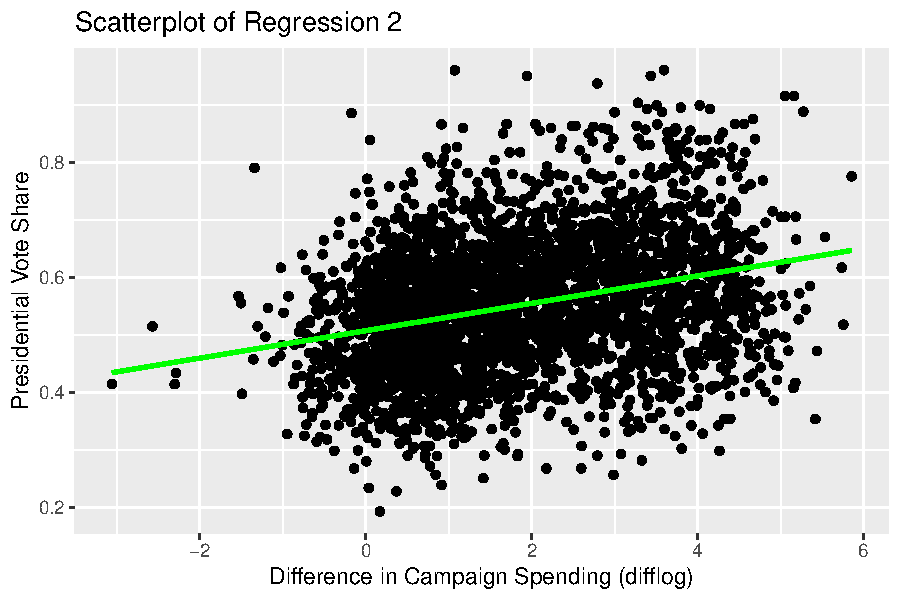
\includegraphics[width=0.85\textwidth]{Scatterplot_of_Regression_2.pdf}
			\caption{Scatterplot of Regression 2}
			\label{fig:scatterplot_regression2}
		\end{figure}
		
		\newpage
		\item Save the residuals of the model in a separate object.	\vspace{0cm}
		
		\begin{lstlisting}
			Save the residuals of the model in a separate object (R).
			residuals_2 <- resid(Regression_2)
		\end{lstlisting}
		
		\item Write the prediction equation.
		
		\begin{align*}
			Y &= B_0 + B_1 \quad \text{(Linear Regression Model)} \\
			\text{Predicted Presidential voteshare} &= 0.507583 + 0.023837 \times \text{difflog} \quad \text{(Specific coefficients)}
		\end{align*}
		
		
	\end{enumerate}
	
	\newpage	
\section*{Question 3}

\noindent We are interested in knowing how the vote share of the presidential candidate of the incumbent's party is associated with the incumbent's electoral success.
	\vspace{.25cm}
	\begin{enumerate}
		\item Run a regression where the outcome variable is \texttt{voteshare} and the explanatory variable is \texttt{presvote}.
			\vspace{0cm}
			
			\begin{lstlisting}[language=R, caption={Regression Model 3 in R}, label={lst:regression_model}]
			#Run a regression model where the outcome variable is voteshare and 
			the explanatory variable is presvote.
			Regression_3 <- lm(voteshare ~ pressvote, data = incumbents_subset)
				
			# Get summary of model with coefficient estimates
			summary(Regression_3)
			\end{lstlisting}
			
			\begin{verbatim}
			Coefficients:
			Estimate Std. Error t value Pr(>|t|)    
			(Intercept) 0.441330   0.007599   58.08   <2e-16 ***
			presvote    0.388018   0.013493   28.76   <2e-16 ***
			---
			Signif. codes:  0 ‘***’ 0.001 ‘**’ 0.01 ‘*’ 0.05 ‘.’ 0.1 ‘ ’ 1
			
			Residual standard error: 0.08815 on 3191 degrees of freedom
			Multiple R-squared:  0.2058,	Adjusted R-squared:  0.2056 
			F-statistic:   827 on 1 and 3191 DF,  p-value: < 2.2e-16
		\end{verbatim}
			
		\item Make a scatterplot of the two variables and add the regression line. 
			\vspace{1cm}
			
	\begin{lstlisting}[language=R, caption={Scatterplot 3 code in R}, label={lst:regression_model}]
	# Create a scatterplot with regression line
	ScatterplotRegression3<-ggplot(incumbents_subset, 
	aes(x = presvote, y = voteshare)) +
	geom_point() +
	geom_smooth(method = "lm", se = FALSE, color = "red") +
	labs(title = "Scatterplot of Regression 3",
	x = "Presidential Vote Share",
	y = "Incumbent Vote Share")
	
	# Save Scatterplot as an image
	ggsave("Scatterplot_of_Regression_3.pdf", 
	plot = ScatterplotRegression3, 
	width = 6, height = 4, units = "in")
	\end{lstlisting}		
			
	\newpage
	\begin{figure}[H]
		\centering
		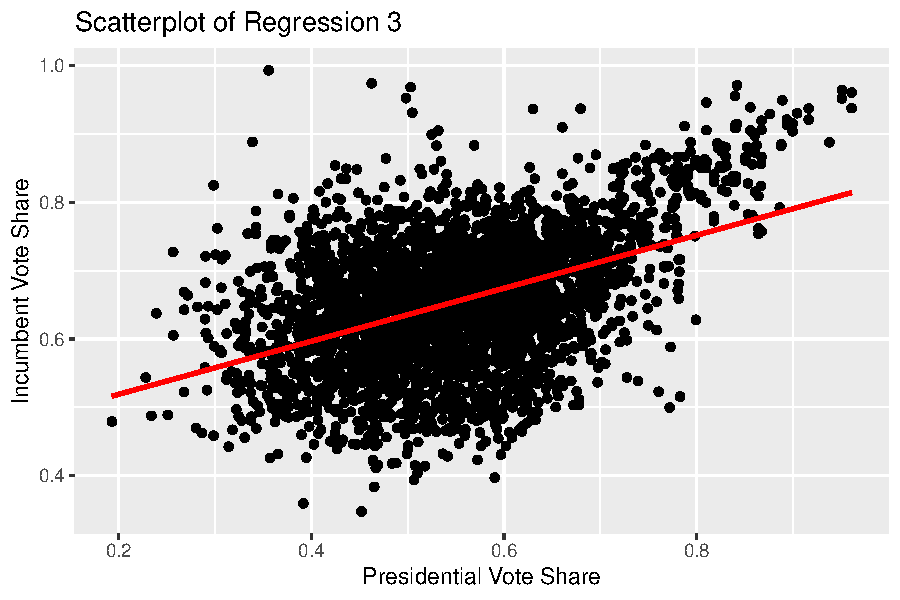
\includegraphics[width=0.85\textwidth]{Scatterplot_of_Regression_3.pdf}
		\caption{Scatterplot of Regression 3}
		\label{fig:scatterplot_regression3}
	\end{figure}
	
		\item Write the prediction equation.
		
		\begin{align*}
			Y &= B_0 + B_1 \quad \text{(Linear Regression Model)} \\
			\text{Pred Incumbent VoteShare} &= 0.441330 + 0.388018 \times \text{Presidential VoteShare} \quad \text{(Specific coefficients)}
		\end{align*}
				
	\end{enumerate}
	

\newpage	
\section*{Question 4}
\noindent The residuals from part (a) tell us how much of the variation in \texttt{voteshare} is $not$ explained by the difference in spending between incumbent and challenger. The residuals in part (b) tell us how much of the variation in \texttt{presvote} is $not$ explained by the difference in spending between incumbent and challenger in the district.
	\begin{enumerate}
		\item Run a regression where the outcome variable is the residuals from Question 1 and the explanatory variable is the residuals from Question 2.	\vspace{0cm}
		
	\begin{lstlisting}[language=R, caption={Regression Model 4 in R}, label={lst:regression_model}]
	#Run a regression with residuals_1 as the outcome and
	residuals_2 as the explanatory variable
	Regression_4_resid <- lm((residuals_1 ~ residuals_2)
	
	# Get summary of model with coefficient estimates
	summary(Regression_4_resid)
	\end{lstlisting}

\begin{verbatim}
	Coefficients:
	Estimate Std. Error t value Pr(>|t|)    
	(Intercept) -5.520e-18  1.299e-03    0.00        1    
	residuals_2  2.569e-01  1.176e-02   21.84   <2e-16 ***
	---
	Signif. codes:  0 ‘***’ 0.001 ‘**’ 0.01 ‘*’ 0.05 ‘.’ 0.1 ‘ ’ 1
	
	Residual standard error: 0.07338 on 3191 degrees of freedom
	Multiple R-squared:   0.13,	Adjusted R-squared:  0.1298 
	F-statistic:   477 on 1 and 3191 DF,  p-value: < 2.2e-16
\end{verbatim}
		
	\item Make a scatterplot of the two residuals and add the regression line. 	\vspace{0cm}
		
	\begin{lstlisting}[language=R, caption={Scatterplot 3 code in R}, label={lst:regression_model}]
		
	ScatterplotRegression4<-ggplot(incumbents_subset, aes(x = residuals_2, y = residuals_1)) +
	geom_point() +
	geom_smooth(method = "lm", se = FALSE, color = "purple") +
	labs(title = "Scatterplot of Regression 4",
	x = "Residuals from Regression 2",
	y = "Residuals from Regression 1")
	
	# Save Scatterplot as an image
	ggsave("Scatterplot_of_Regression_4.pdf", 
	plot = ScatterplotRegression4, 
	width = 6, height = 4, units = "in")	
	\end{lstlisting}			
	
	\newpage	
	
	\begin{figure}[H]
		\centering
		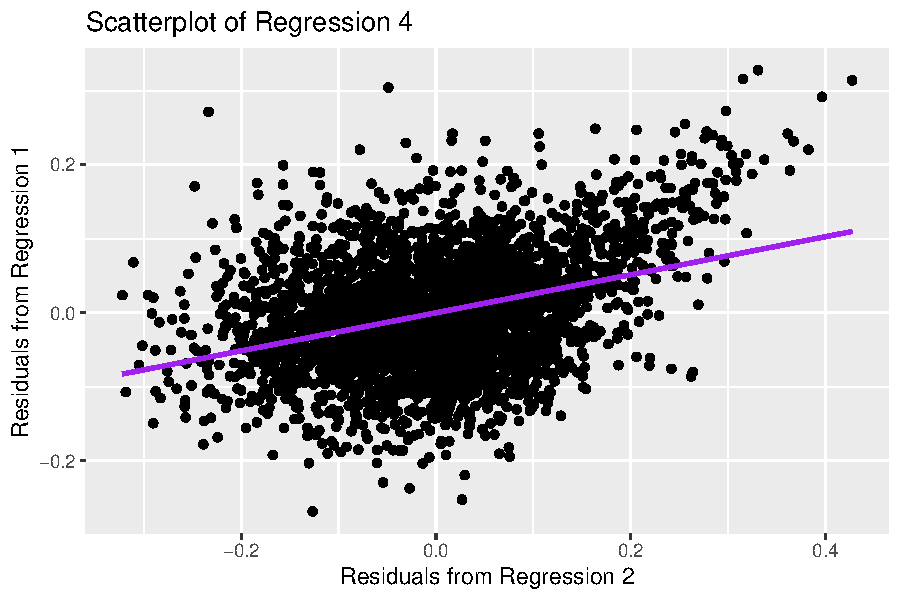
\includegraphics[width=0.85\textwidth]{Scatterplot_of_Regression_4.pdf}
		\caption{Scatterplot of Regression 4}
		\label{fig:scatterplot_regression4}
	\end{figure}
	
	\item Write the prediction equation.
	\begin{align*}
	Y &= B_0 + B_1 \quad \text{(Linear Regression Model)} \\
	\text{Resid from Regression 1} &= -5.520 + 2.569 \times \text{Resid from Regression 2} \quad \text{(Specific coefficients)}
	\end{align*}	
	
	
	\end{enumerate}
	
	\newpage	

\section*{Question 5}
\noindent What if the incumbent's vote share is affected by both the president's popularity and the difference in spending between incumbent and challenger? 
	\begin{enumerate}
		\item Run a regression where the outcome variable is the incumbent's \texttt{voteshare} and the explanatory variables are \texttt{difflog} and \texttt{presvote}.	\vspace{0cm}
		
		\begin{lstlisting}[language=R, caption={Regression Model 5 in R}, label={lst:regression_model}]
		#Run a regression where the outcome variable is the incumbent's voteshare and the explanatory variables are difflog and presvote.
		Regression_5 <- lm(voteshare ~ difflog + presvote, data = incumbents_subset)
			
		# Get summary of model with coefficient estimates
		summary(Regression_5)
		\end{lstlisting}
		
		\begin{verbatim}
		Coefficients:
		Estimate Std. Error t value Pr(>|t|)    
		(Intercept) 0.4486442  0.0063297   70.88   <2e-16 ***
		difflog     0.0355431  0.0009455   37.59   <2e-16 ***
		presvote    0.2568770  0.0117637   21.84   <2e-16 ***
		---
		Signif. codes:  0 ‘***’ 0.001 ‘**’ 0.01 ‘*’ 0.05 ‘.’ 0.1 ‘ ’ 1
		
		Residual standard error: 0.07339 on 3190 degrees of freedom
		Multiple R-squared:  0.4496,	Adjusted R-squared:  0.4493 
		F-statistic:  1303 on 2 and 3190 DF,  p-value: < 2.2e-16
			\end{verbatim}
		
		\item Write the prediction equation.	\vspace{0cm}
			
		\begin{align*}
		Y &= B_0 + B_1X_1 + B_2X_2 \quad \text{(Multiple Linear Regression Model)} \\
		\text{Incumbent's Voteshare} &= 0.4486 + 0.0355 \cdot \text{difflog} + 0.2568 \cdot \text{presvote}
		\end{align*}
		
		\item What is it in this output that is identical to the output in Question 4? Why do you think this is the case?
		
		The residual standard errors (RSE) are almost identical 0.07338 for Regression 4
		and 0.07339 for Regression 5, this could occur because...
		
	\end{enumerate}




\end{document}
